\chapter{Compiler Overview}\label{Chp:CompilerOverview}
Most compilers are either a multi-pass or a single-pass compiler. 
Each have their advantages and disadvantages however the most significant difference is that in a single-pass compiler, as the name suggests, only one does one pass of the source code. \todo{or other representations of the source code, such as pt or ast? -- Troels}
This highly limits the information available to the compiler and this decreases the odds of creating efficient programs, which is not wished for in \gls{gamble}. \todo{Informationen er vel den samme, men der er mindre mulighed for advancerede checks og/eller optimeringer? -- Troels}
As such the \gls{gamble} compiler will be a multi-pass compiler and can therefore be divided into phases.
In this chapter the different phases of the compiler and their goals and tasks will be presented to give an overview for the chapters to come.

The compiler for \gls{gamble} is separated into three phases: syntax analysis, contextual analysis and code generation.
\myref{fig:phases} shows a state diagram of the phases of the compiler.
Syntax analysis and contextual analysis transforms the source code into an intermediate representation, and verifies the source code according to the syntax specified in the \acrshort{cfg} and also for type as well as scope and type checking.
Java 1.8 is chosen as the language the compiler will be written in, which is the language used in the languages and compiler course.
When making a compiler an object-oriented language simplifies many tasks because of encapsulation, polymorphism and inheritance. 
The paradigm allows for many structural options, and reuse of code when inheriting, which would be difficult using another paradigm like imperative or functional programming.
Java also works across platforms, which is a useful feature.

\begin{figure}[ht]
\centering
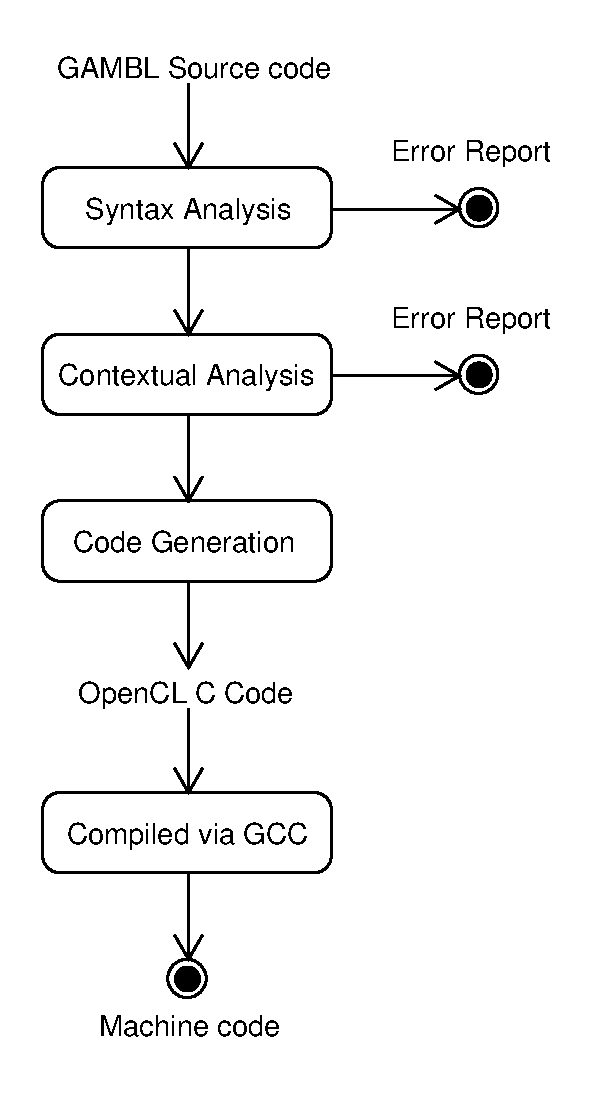
\includegraphics[width=0.35\textwidth]{figures/ClassDiagrams/CompilerDiagram.pdf}
\caption{State diagram showing the phases of the compiler when it takes \gls{gamble} source code and compiles it into machine code.}\label{fig:phases}
\end{figure}

In the syntax analysis phase the input source code is parsed and separated into tokens according to the \acrshort{cfg}.
This is done by the scanner, the parser structures these tokens into a tree structure, which can be traversed in the path the source code is written.
When the source code has been parsed the tree is then simplified to remove unnecessary information such that a tree with less nodes can be traversed.
If a syntactical error is found in this phase the compiler stops and reports errors in the console.

In the contextual analysis phase the tree is used to generate a table, containing all the variables and functions which is declared in the source code.
This is called a symbol table, and it is used to check if the variables and functions called and used in the source code are in scope, and also if they uphold the type rules of \gls{gamble}.
If one or more errors are found in this phase the compiler will stop compilation, and report the errors to the programmer, not just what is wrong but also where the error is located.
If no errors are found it results in the tree now containing additional information about the types of expressions in the source code, and it continues to the next phase.

The last phase of the compiler is code generation and optimisation.
Optimisation is defined\todo{af os eller generelt? -- Troels} as any process which will make the generated program's runtime faster, e.g. adding constant numbers before the runtime etc, or changing the order of access to matrices to increase locality. \todo{Det er fint at have det med, men vi optimere jo ikke på noget, så ved ikke om det hører til her ?? - Søren}
In the code generation phase the output code is generated from all the information gathered from the previous phases of the compiler.

The target language of this compiler is OpenCL C.
To compile OpenCL C code additional software for the GPU is required, depending on the machine the path to this software may be required when compiling, as such one cannot simply run this on all machines.
By compiling the OpenCL C code, it is translated into machine code and linked with libaries, which the computer then understands.\todo{Skal vi skrive et afsnit efter code gen som hedder noget med:How to run a \gls{gamble} program? - Søren Dette kunne være under makefile tingene? -- Troels}
This is an abstraction made by the project group to simplify the process of generating code, as targeting the \acrshort{gpu} using its specific instruction set, not only gives problems targeting more types of GPUs but is also too demanding for the project group to understand let alone use in just one semester.
OpenCL C is low level compared to Java or C\#, and C has even been characterised as a portable assembly language, as many features of the language translates closely to assembly. \citep{CPort}\todo{Hvilket er relevant fordi? - Marc .. Det er et valg vi har truffet og diskutere senere. -- Troels}

\myref{fig:tombstone} shows a tombstone diagram of the translations of \gls{gamble} for this compiler.
The compiler takes the \gls{gamble} source code as input and translates it into OpenCL C using a compiler written in Java, the OpenCL C code is then compiled using a C compiler written in C, and outputs machine code which can be run by the computer.\todo[inline]{hvad med kernels som bliver jit compiled? MP Det gør de ikke nødvendigvis, men vi kunne tilføje at ``this diagram excludes the kernels'' -- Troels}
\begin{figure}[!ht]
\centering
\begin{tikzpicture}
\matrix (m) [matrix of nodes,%nodes={minimum width=1em,minimum height=1.7em}
            ]
{
 \gls{gamble}  & $\to$ &  OpenCL C  \\
    &  Java    & OpenCL C & $\to$ & \hspace{1 em} M \hspace{2 em}  \\
    &       &   & C  &         \\
    &       &               \\
  };
 \draw (m-1-1.south west) |- (m-1-3.north east) |- (m-2-2.north east) |- (m-2-2.south west) |- (m-1-1.south west);
\draw (m-2-2.south east) |- (m-2-5.north east) --(m-2-5.south east) -- (m-2-5.south west) |- (m-3-4.south west) |- (m-2-2.south east);

\end{tikzpicture}
\caption{Tombstone diagram for the compiler.}
\label{fig:tombstone}
\end{figure}


The overall structure of the compiler is also implemented using these phases as seen on \myref{fig:compilerOverview} where the \texttt{main} method of the \texttt{Main} class calls the different phases.
This separation helps give an overview when working with the compiler, all the phases are distinctly separated, this seperation is helpful when making changes as a change in one phase will not conflict with other phases it also helps locate where in the compiler changes are required.

\begin{figure}[!ht]
	\begin{sideways}
	%\fbox{
		\begin{minipage}{18cm}
			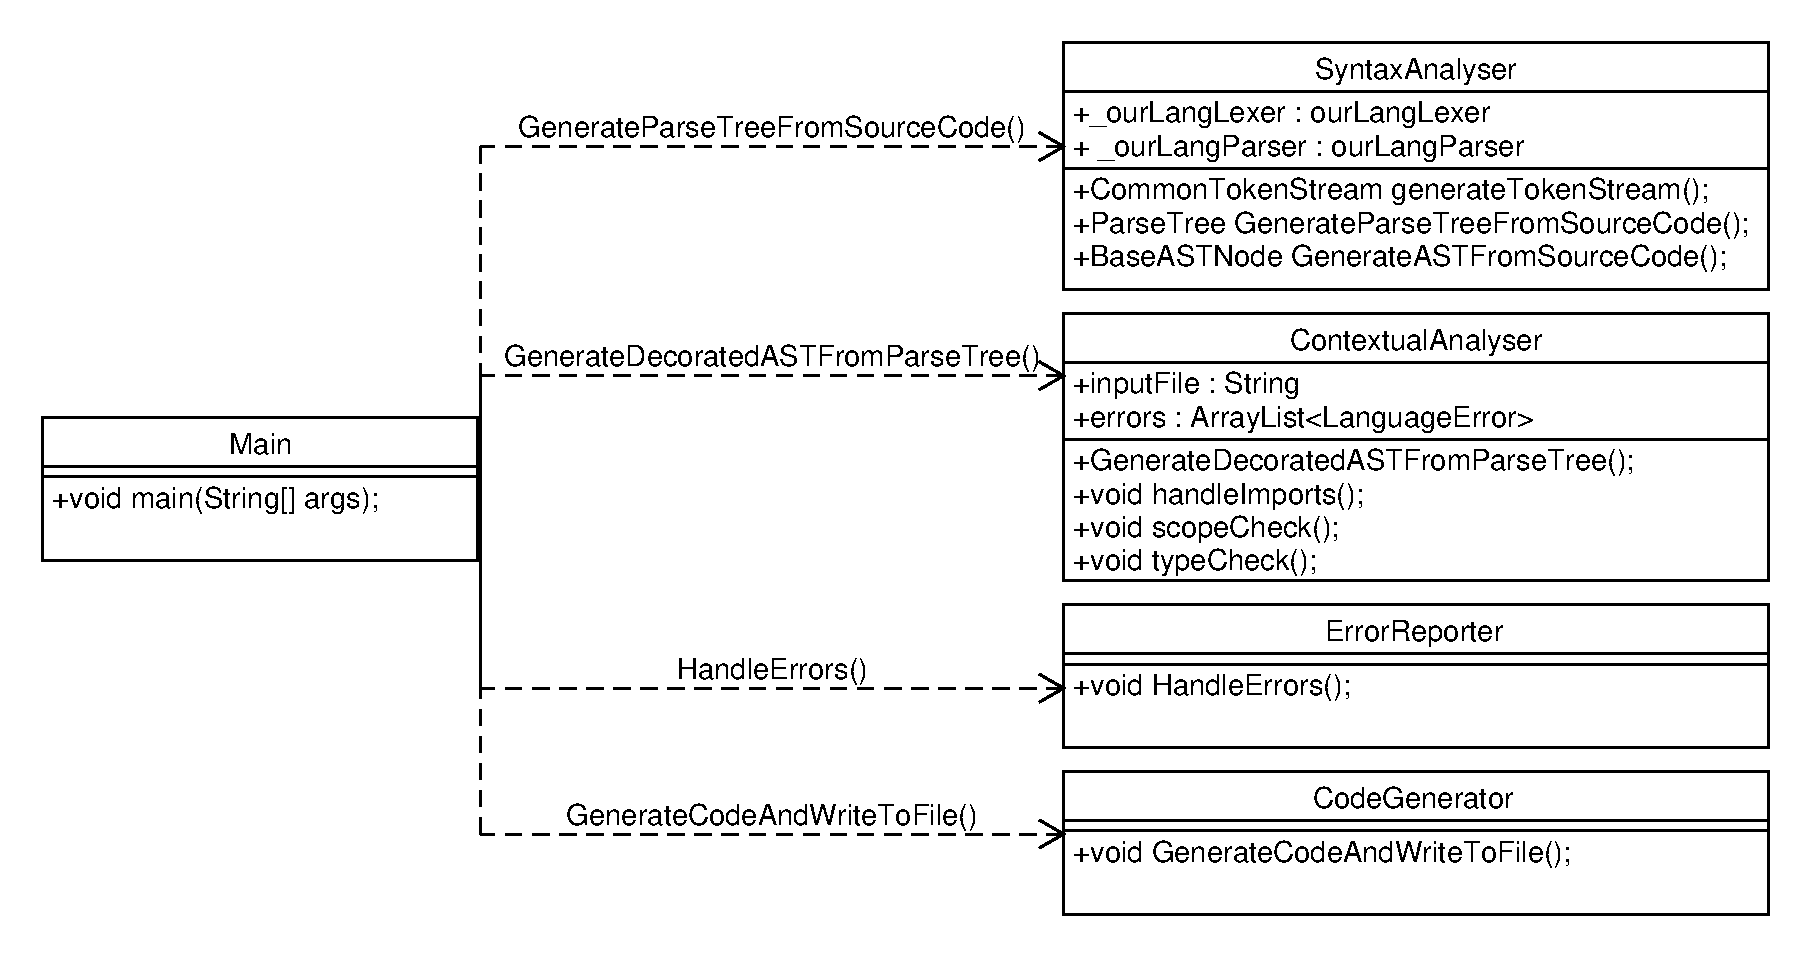
\includegraphics[height=0.42\textheight]{figures/ClassDiagrams/DiagramOfCallsFromMain.pdf}
		\end{minipage}
	%	}
	\end{sideways}
	\centering
	\caption{Diagram showing the structure of the compiler by showing the \texttt{main()} method's method calls. Arguments are omitted for simplicity}\label{fig:compilerOverview}
\end{figure}
\todo{figuren viser prettyprint hvilket ikke er dækket i ovenstående tekst, bør der måske være lidt om dette? - Marc}

\clearpage

\label{SourceCodeAsTrees}
\todo{Write about Sourcecode as Trees, and why we do that.}

